\section{Auswertung}
\label{sec:Auswertung}

\subsection{Wheatstone-Brücke}
Für die Messung des Widerstandes (Wert 11) wurden drei Messreihen vorgenommen, bei denen $R_2$ variiert wurde und das Potentiometer($R_3, R_4=1\si{\kilo}\si{\ohm}-R_3$) abgestimmt wurde, sodass ein Spannungsminimum entsteht. Die eingesetzten, gemessenen und berechneten  Widerstände wurden in \autoref{tab:WS} aufgelistet. Der Widerstand $R_x$ kann mit diesen Werten nach \autoref{eqn:wheatstone-rx} berechnet werden.

Mit der für das Potentiometer (also für $R_3/R_4$) gegebenen Messungenauigkeit von $0.5\%$ und der Standardabweichung für $R_x$ von $\sigma_{R_x}=1.92 \si{\ohm}$ lässt sich auch ein Fehler bestimmen. Für $R_x$ ergibt sich dann: 

\begin{align}
  R_x=R_{11}=(490.9 \pm 3.6)\si{\ohm}
\end{align}

\begin{table}
  \centering
  \caption{Daten zur Wheatstone-Brücke}
  \label{tab:WS}
  \sisetup{table-format=2.1}
  \begin{tabular}{c c c c}
  \toprule
  $R_2 \, [\si{\ohm}]$ &$R_3 \, [\si{\ohm}]$ &$R_4 \, [\si{\ohm}]$ & $R_x \, [\si{\ohm}]$\\
  \midrule
   664 & 425.25 & 574.75& 491.285\\
   1000 & 330 & 670 & 492.537 \\
   332 & 595.5 & 404.5 & 488.766 \\
  \bottomrule
  \end{tabular}
\end{table}
%\newpage
\subsection{Kapazitätsmessbrücke}
\label{sec:akap}
In \autoref{sec:theorie-kapazitaetsmessbruecke} wurde bereits beschrieben, wie die Kenndaten eines Kondensators mit einer Kapazitätsmessbrücke bestimmt werden können. Es wurden 2 RC-Kombinationen (Werte 8 und 9) und ein Kondensator (Wert 3) ausgemessen. Die Kenndaten wurden nach \autoref{eqn:values-kapazitaeten} berechnet.
Für die Werte der verlustbehafteten Kondensatoren ergibt sich dann:

\begin{align}
  C_8&=(301.73 \pm 3.24)\si{\nano} \si{\farad}\\
  R_8&=(640.12 \pm 25.85) \si{\ohm}
\end{align}
und
\begin{align}
  C_9&=(193.19 \pm 58.88)\si{\nano} \si{\farad}\\
  R_9&=(14.95 \pm 7.50)\si{\kilo} \si{\ohm}
\end{align}
Die Ergebnisse für Wert 9 werden in \autoref{sec:Diskussion} diskutiert. 
Für den Wert des Kondensators (Wert 3) ergibt sich:
\begin{align}
  C_3&=(434.94 \pm 8.32)\si{\nano} \si{\farad}
\end{align}

\subsection{Induktivitätsmessbrücke}
 Die Bestimmung der Kenndaten einer Spule mit einer Induktivitätsmessbrücke wurde in \autoref{sec:theorie-induktivitätsmessbrücke} beschrieben. Die erhaltenen Messdaten wurden in \autoref{tab:ind} aufgelistet.
\begin{table}
  \centering
  \caption{Messdaten zur Induktivitätsmessbrücke}
  \label{tab:ind}
  \sisetup{table-format=2.1}
  \begin{tabular}{c c c}
  \toprule
  $R_2 \, [\si{\ohm}]$ &$R_3 \, [\si{\ohm}]$ &$L_2 \, [\si{\milli} \si{\henry}]$\\
  \midrule
   65 & 711 & 20.1\\
   54 & 646 & 14.6 \\
   96 & 499 & 27.5 \\
  \bottomrule
  \end{tabular}
\end{table}
%\newpage
Mit  \autoref{tab:ind} lassen sich nach \autoref{eqn:values-induktivitaetsbruecke} Induktivität und Verlustwiderstand der unbekannten Spule berechnen. Es ergeben sich:
\begin{align}
  L_{19}&=(34.49 \pm 7.65)\si{\milli} \si{\henry}\\
  R_{19}&=(118.02 \pm 24.55)\si{\ohm}
\end{align}

\subsection{Maxwell-Brücke}
Mit einer Maxwell-Brücke wurden die Daten zu Wert 19 dann nochmal bestimmt(Messdaten siehe \autoref{tab:max}). 
\begin{table}
  \centering
  \caption{Messdaten zur Maxwell-Brücke}
  \label{tab:max}
  \sisetup{table-format=2.1}
  \begin{tabular}{c c c c}
  \toprule
  $R_2 \, [\si{\ohm}]$ &$R_3 \, [\si{\ohm}]$ &$R_4 \, [\si{\ohm}]$&$C_4 \, [\si{\nano} \si{\farad}]$\\
  \midrule
  1000 & 26 & 230 & 992\\
  332  & 84.5 & 245 & 992\\
  332 & 139 & 400 & 597\\
  664 & 69 & 403.5 & 597\\
  \bottomrule
  \end{tabular}
\end{table}
%\newpage
Als Toleranz der variaben Widerstände $R_3$ und $R_4$ waren hier $3\%$ angegeben.
Mit  \autoref{tab:max} lassen sich nach \autoref{eqn:kenngroessen-maxwell} Induktivität und Verlustwiderstand der unbekannten Spule dann ein zweites Mal berechnen. Es ergeben sich:
\begin{align}
  L_{19Mw}&=(27.13 \pm 1.27)\si{\milli} \si{\henry}\\
  R_{19Mw}&=(114.12 \pm 5.36)\si{\ohm}
\end{align}


\subsection{Wien-Robinson-Brücke}
Wie in \autoref{fig:mess} zu sehen ergab sich für die Wien-Robinson-Brücke eine Messreihe von Brückenspannungen mit dazugehörigen Frequenzen.Bei der Auswertung der Wien-Robinson-Brücke konnte aus den Messdaten eine Frequenz $f_0$ bei der die Brückenspannung minimal wurde bestimmt werden. Hier ergab sich eine Frequenz $f_0=160 \si{\hertz}$ mit einer Brückenspannung von $U_{Br,Min}=11.1 \si{\milli} \si{\volt}$. Die theoretische Kreisfrequenz für die minimale Brückenspannung nach \autoref{eqn:wien-robinson-w0} liegt bei $\omega_0=\frac{1}{RC}=1006\si{\hertz}$ (dies entspricht als auf die Zeit bezogene Frequenz $(1006/2\pi)\si{\hertz}=160.11\si{\hertz}$) und liegt somit sehr nahe an dem gemessenen Wert für $f_0$. In \autoref{fig:plot} wurden die Messdaten geplottet. Dabei wurde der Quotient $U_{Br}/U_S$ in einem halblogarithmischen Diagramm gegen $\Omega=f/f_0$ aufgetragen. Die Theorie-Kurve wurde dabei aus \autoref{eqn:wien-robinson-abgleich-einfach} berechnet.
\begin{figure}
  \centering
  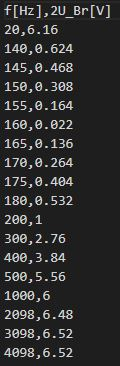
\includegraphics{daten/WienR.JPG}
  \caption{Messdaten zur Wien-Robinson-Brücke}
  \label{fig:mess}
\end{figure}


\begin{figure}
  \centering
  \includegraphics{WRplot.pdf}
  \caption{Halblogarithmische Darstellung der Frequenzabhängigkeit der Brückenspannung der Wien-Robinson-Brücke}
  \label{fig:plot}
\end{figure}
\newpage

\subsection{Klirrfaktor}
Der Klirrfaktor k kann anschließend, wie in \autoref{sec:klirrfaktor} beschrieben, berechnet werden. Zuerst muss dafür $U_2$ nach nach \autoref{eqn:klirrfaktor-u2} berechnet werden. $f(2)$ bezieht sich dabei auf \autoref{eqn:wien-robinson-abgleich-einfach}. Es ergibt sich für $U_2$:
\begin{align}
U_2&=\frac{0.0111\si{\volt}}{f(2)}\\
U_2&=0.4995\si{\volt}
\end{align}
Nun kann man $U_2$ in \autoref{eqn:klirrfaktor} einsetzen, um k zu bestimmen($U_1=10\si{\volt}$):
\begin{align}
  k&=\frac{U_2}{U_1}\\
  k&=0.04995\\
  k&=5\%
\end{align}
\newpage  
